% This LaTeX was auto-generated from MATLAB code.
% To make changes, update the MATLAB code and export to LaTeX again.

\documentclass{article}

\usepackage[utf8]{inputenc}
\usepackage[T1]{fontenc}
\usepackage{lmodern}
\usepackage{graphicx}
\usepackage{color}
\usepackage{hyperref}
\usepackage{amsmath}
\usepackage{amsfonts}
\usepackage{epstopdf}
\usepackage[table]{xcolor}
\usepackage{matlab}

\sloppy
\epstopdfsetup{outdir=./}
\graphicspath{ {./Geometry_images/} }

\begin{document}

\begin{matlabcode}
%Dimensions of the House


xStart = 0%Ignored Base is ALWAYS (0|0) for Symmetry Reasons
\end{matlabcode}
\begin{matlaboutput}
xStart = 0
\end{matlaboutput}
\begin{matlabcode}
yStart = 0
\end{matlabcode}
\begin{matlaboutput}
yStart = 0
\end{matlaboutput}
\begin{matlabcode}
height = 8
\end{matlabcode}
\begin{matlaboutput}
height = 18
\end{matlaboutput}
\begin{matlabcode}
width = 8
\end{matlabcode}
\begin{matlaboutput}
width = 8
\end{matlaboutput}
\begin{matlabcode}
margin = 0.5
\end{matlabcode}
\begin{matlaboutput}
margin = 0.5000
\end{matlaboutput}
\begin{matlabcode}

%Critical Point
xC = 4;
yC = 4;


%Door
doorW = 1
\end{matlabcode}
\begin{matlaboutput}
doorW = 1
\end{matlaboutput}
\begin{matlabcode}
doorH = 2
\end{matlabcode}
\begin{matlaboutput}
doorH = 2
\end{matlaboutput}
\begin{matlabcode}

%Window
windW = 1.5;
windH = 1.5;
windMargin = 0.25;

	%Helping Variables
	ww = windW + 2 * windMargin %window Width and margin
\end{matlabcode}
\begin{matlaboutput}
ww = 2
\end{matlaboutput}
\begin{matlabcode}
	wh = windH + 2 * windMargin
\end{matlabcode}
\begin{matlaboutput}
wh = 2
\end{matlaboutput}
\begin{matlabcode}
	%For House
	rw = width - 2 * margin %real width
\end{matlabcode}
\begin{matlaboutput}
rw = 7
\end{matlaboutput}
\begin{matlabcode}
	rh = height - margin %real height
\end{matlabcode}
\begin{matlaboutput}
rh = 17.5000
\end{matlaboutput}
\begin{matlabcode}
    
%Step Size
doorStep = 10
\end{matlabcode}
\begin{matlaboutput}
doorStep = 8
\end{matlaboutput}
\begin{matlabcode}
windowStep = 3
\end{matlabcode}
\begin{matlaboutput}
windowStep = 1
\end{matlaboutput}
\begin{matlabcode}


data = 0;
DataMatrix = zeros(2,5);

%Steps always begin with 0:step
maxDStep = floor((rw - doorW)/doorStep)
\end{matlabcode}
\begin{matlaboutput}
maxDStep = 0
\end{matlaboutput}
\begin{matlabcode}
maxWindowStepWidth = floor((rw - ww)/windowStep)
\end{matlabcode}
\begin{matlaboutput}
maxWindowStepWidth = 5
\end{matlaboutput}
\begin{matlabcode}
maxWindowStepHeight = floor((rh - doorH - wh)/windowStep)
\end{matlabcode}
\begin{matlaboutput}
maxWindowStepHeight = 13
\end{matlaboutput}
\begin{matlabcode}
maxWStep = (maxWindowStepWidth+1) * (maxWindowStepHeight+1) - 1 %+ maxWindowStepWidth//2
\end{matlabcode}
\begin{matlaboutput}
maxWStep = 83
\end{matlaboutput}
\begin{matlabcode}

nextPosW = ceil(ww/windowStep)
\end{matlabcode}
\begin{matlaboutput}
nextPosW = 2
\end{matlaboutput}
\begin{matlabcode}
nextPosH = ceil(wh/windowStep)
\end{matlabcode}
\begin{matlaboutput}
nextPosH = 2
\end{matlaboutput}
\begin{matlabcode}

%Plot
plotSquare(xStart, yStart, width, height,[0 0 0]);
hold on
plotSquare(xStart + margin,yStart,rw,rh,'r'); %Margin
plot(xC,yC,'go')

%Find all possible configurations
for d = 0:1:maxDStep
    doorX = margin + d * doorStep;
    for w1 = 0:1:maxWStep
        colW1 = mod(w1,maxWindowStepWidth+1);
        rowW1 = floor(w1/(maxWindowStepWidth+1)); 
        windX = colW1*windowStep + margin + windMargin + 0.1 * rand();
        windY = rh -wh-rowW1*windowStep + windMargin + 0.1 * rand();
        

        for w2 = w1+nextPosW:1:maxWStep
            %Misses some data points at the turnover point
            
            colW2 = mod(w2,maxWindowStepWidth+1);
            rowW2 = floor(w2/(maxWindowStepWidth+1));
           
            if rowW1 == rowW2 || rowW2 - rowW1 >= nextPosH %Else a window *COULD* overlap
            
            windX2 = colW2*windowStep + margin + windMargin + 0.1 * rand();
            windY2 = rh -wh -rowW2*windowStep + windMargin + 0.1 * rand();
            
            
            %Stop if window would be inside critical point
            if isInRectangle(windX,windY,windW,windH,xC,yC) || ...
                    isInRectangle(windX2,windY2,windW,windH,xC,yC)
               
            else
                %Plotting
                plotSquare(doorX,yStart, doorW, doorH, [0.5 0.5 0.5]);
                plotSquare(windX, windY, windW, windH, [0.2 1 0.2]);
                plotSquare(windX2, windY2, windW, windH, [0.2 0.2 0.5]);  
                
                data = data + 1;
                DataMatrix(data,:) = [doorX windX windY windX2 windY2];
                
                axis([-1 9 -0.5 8.5])
            end
            end
            
            
            
        end
    end
end

            
axis([-1 9 -0.5 8.5])
data
\end{matlabcode}
\begin{matlaboutput}
data = 196
\end{matlaboutput}
\begin{matlabcode}
hold off
\end{matlabcode}
\begin{center}
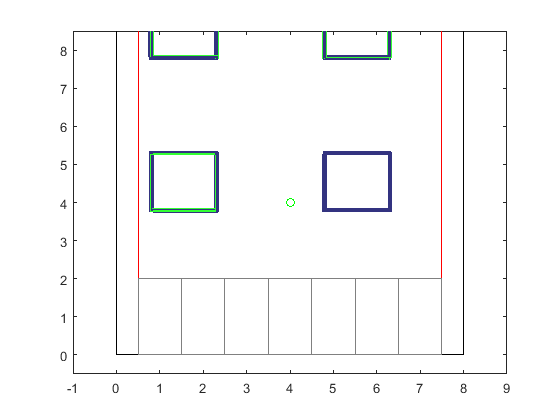
\includegraphics[width=\maxwidth{56.196688409433015em}]{figure_0.png}
\end{center}


\vspace{1em}
\begin{par}
\begin{flushleft}
Does not check, if door is in critical point
\end{flushleft}
\end{par}


\vspace{1em}
\begin{par}
\begin{flushleft}
*IF, door,LE,3,THEN
\end{flushleft}
\end{par}

\begin{par}
\begin{flushleft}
	*IF, w1, GE, 12, THEN
\end{flushleft}
\end{par}

\begin{par}
\begin{flushleft}
	colW1 = colW1 + 2
\end{flushleft}
\end{par}

\begin{par}
\begin{flushleft}
	*ELSE
\end{flushleft}
\end{par}

\begin{par}
\begin{flushleft}
	*ENDIF
\end{flushleft}
\end{par}

\begin{par}
\begin{flushleft}
	!Same for w2
\end{flushleft}
\end{par}

\begin{par}
\begin{flushleft}
	*IF, w2, GE, 12, THEN
\end{flushleft}
\end{par}

\begin{par}
\begin{flushleft}
	colW2 = colW2 + 2
\end{flushleft}
\end{par}

\begin{par}
\begin{flushleft}
	*ELSE
\end{flushleft}
\end{par}

\begin{par}
\begin{flushleft}
	*ELSE
\end{flushleft}
\end{par}

\begin{par}
\begin{flushleft}
	*ENDIF
\end{flushleft}
\end{par}

\end{document}
